% =====================================================================
%  Tier 1.1 Manipulation Skill — Autoregressive Motion Primitive Paradigm
%  Compile:  pdflatex manip_primitive_arch.tex
%  Output:   manip_primitive_arch.pdf
% =====================================================================
\documentclass[tikz, border=4pt]{standalone}
\usepackage{tikz}
\usepackage{xcolor}
\usepackage{amsmath, amssymb}
\usetikzlibrary{positioning, arrows.meta, shapes.geometric, fit, backgrounds, calc}

% --- color-blind-friendly palette (Wong 2011 inspired) ---
\definecolor{cInputFill}{HTML}{B3D9F2}
\definecolor{cInputEdge}{HTML}{4A90C9}
\definecolor{cDispFill}{HTML}{FFE7A6}
\definecolor{cDispEdge}{HTML}{C8932E}
\definecolor{cPrimFill}{HTML}{FFD9B3}
\definecolor{cPrimEdge}{HTML}{C97A1E}
\definecolor{cModelFill}{HTML}{B3E5D8}
\definecolor{cModelEdge}{HTML}{2D8F77}
\definecolor{cVadFill}{HTML}{D9C2F0}
\definecolor{cVadEdge}{HTML}{7C56B5}
\definecolor{cOutFill}{HTML}{E0E0E0}
\definecolor{cOutEdge}{HTML}{606060}

\begin{document}
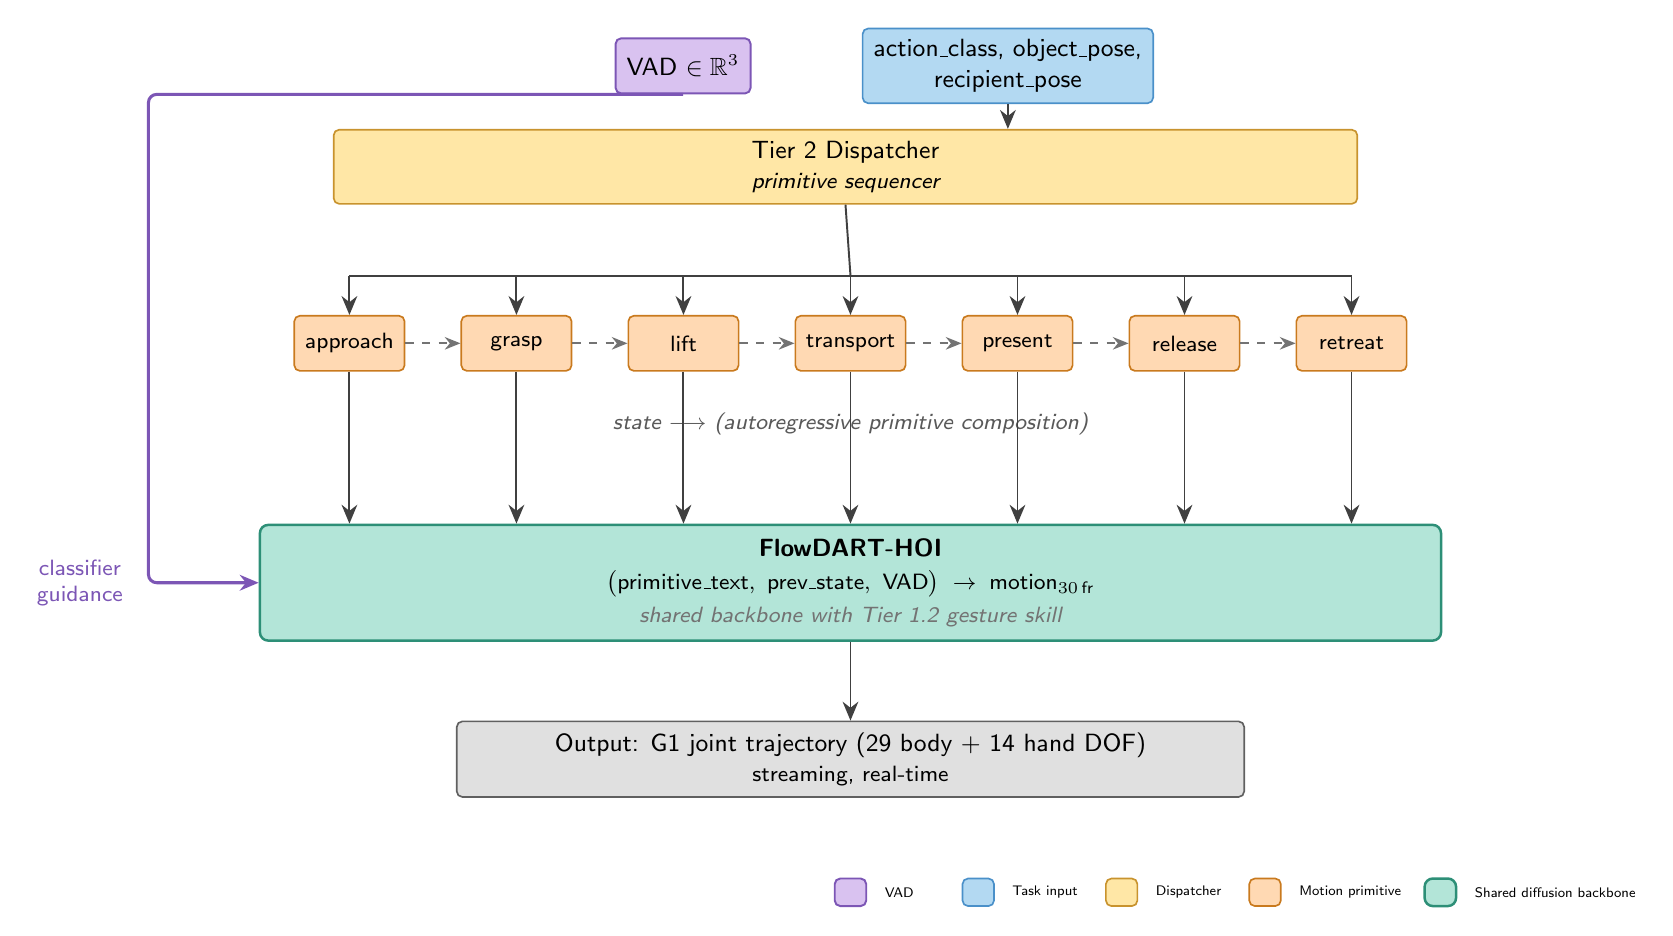
\begin{tikzpicture}[
    font=\sffamily\small,
    inbox/.style    ={rectangle, rounded corners=2pt, draw=cInputEdge, fill=cInputFill, line width=0.6pt, minimum height=7mm, align=center, inner sep=4pt},
    vadbox/.style   ={rectangle, rounded corners=2pt, draw=cVadEdge,  fill=cVadFill,   line width=0.7pt, minimum height=7mm, align=center, inner sep=4pt},
    dispbox/.style  ={rectangle, rounded corners=2pt, draw=cDispEdge, fill=cDispFill,  line width=0.6pt, minimum height=8mm, align=center, inner sep=4pt},
    primbox/.style  ={rectangle, rounded corners=2pt, draw=cPrimEdge, fill=cPrimFill,  line width=0.6pt, minimum width=14mm, minimum height=7mm, align=center, inner sep=2pt, font=\sffamily\footnotesize},
    modelbox/.style ={rectangle, rounded corners=3pt, draw=cModelEdge, fill=cModelFill, line width=0.9pt, minimum height=14mm, align=center, inner sep=5pt},
    outbox/.style   ={rectangle, rounded corners=2pt, draw=cOutEdge,  fill=cOutFill,   line width=0.6pt, minimum height=7mm, align=center, inner sep=4pt},
    arr/.style      ={-{Stealth[length=2.4mm, width=2mm]}, line width=0.7pt, black!75},
    autoarr/.style  ={-{Stealth[length=2mm,   width=1.6mm]}, line width=0.6pt, dashed, black!55},
    vadarr/.style   ={-{Stealth[length=2.4mm, width=2mm]}, line width=1.1pt, cVadEdge}
]

% ===== Row 1: Inputs =====
\node[vadbox] (vad) {VAD $\in \mathbb{R}^3$};
\node[inbox, right=14mm of vad] (task) {action\_class,\ object\_pose,\\ recipient\_pose};

% ===== Row 2: Dispatcher =====
\coordinate (anchor) at ($(vad)!0.5!(task)$);
\node[dispbox, below=8mm of anchor, minimum width=130mm] (disp) {Tier 2 Dispatcher\\\footnotesize\itshape primitive sequencer};
\draw[arr] (task.south) -- (disp.north -| task);

% ===== Row 3: Primitive sequence =====
% FIX P1: primitive spacing 2mm → 7mm so autoregressive arrows are visible
\node[primbox, below=14mm of disp.south, xshift=-63mm] (p1) {approach};
\node[primbox, right=7mm of p1] (p2) {grasp};
\node[primbox, right=7mm of p2] (p3) {lift};
\node[primbox, right=7mm of p3] (p4) {transport};
\node[primbox, right=7mm of p4] (p5) {present};
\node[primbox, right=7mm of p5] (p6) {release};
\node[primbox, right=7mm of p6] (p7) {retreat};

% Dispatcher fan-out via horizontal bar
\coordinate (busy) at ($(p4.north)+(0,5mm)$);
\draw[line width=0.7pt, black!75] (disp.south) -- (busy);
\draw[line width=0.7pt, black!75] (p1.north |- busy) -- (p7.north |- busy);
\foreach \p in {p1,p2,p3,p4,p5,p6,p7} {
  \draw[arr] (\p.north |- busy) -- (\p.north);
}

% FIX P1: autoregressive arrows now span 7mm — visible
\foreach \i/\j in {1/2, 2/3, 3/4, 4/5, 5/6, 6/7} {
  \draw[autoarr] (p\i.east) -- (p\j.west);
}
% FIX P3: state label — footnotesize, below the primitive row, centered, with arrow
\node[font=\sffamily\footnotesize\itshape, black!65, below=4mm of p4]
     (statelabel) {state $\longrightarrow$ (autoregressive primitive composition)};

% ===== Row 4: Generator =====
\node[modelbox, below=10mm of statelabel, minimum width=150mm] (gen) {%
  \textbf{FlowDART-HOI} \\[1pt]
  \footnotesize $\bigl(\text{primitive\_text},\ \text{prev\_state},\ \text{VAD}\bigr) \;\rightarrow\; \text{motion}_{30\,\text{fr}}$ \\[1pt]
  \footnotesize\itshape\textcolor{black!55}{shared backbone with Tier 1.2 gesture skill}
};

\foreach \p in {p1,p2,p3,p4,p5,p6,p7} {
  \draw[arr] (\p.south) -- (gen.north -| \p);
}

% FIX P2 (round 3): VAD curve as clean 3-segment L (LEFT → DOWN → RIGHT) with
%   rounded corners. Path runs entirely in the left margin — never overlaps
%   the dispatcher, primitive row, or any other box.
\coordinate (vadwp)       at ($(gen.west) + (-14mm, 0)$);          % bottom-left corner
\coordinate (vadabovewp)  at (vadwp |- vad.south);                  % top-left corner
\draw[vadarr, rounded corners=3pt]
     (vad.south) -- (vadabovewp) -- (vadwp) -- (gen.west);
\node[font=\sffamily\footnotesize, cVadEdge, align=center, anchor=east]
     at ($(vadwp) + (-2mm, 0)$) {classifier\\guidance};

% ===== Row 5: Output =====
\node[outbox, below=10mm of gen, minimum width=100mm] (out) {%
  Output: G1 joint trajectory (29 body + 14 hand DOF)\\
  \footnotesize streaming, real-time
};
\draw[arr] (gen.south) -- (out.north);

% ===== Legend (small, bottom) =====
\begin{scope}[shift={($(out.south)+(0,-12mm)$)}, font=\sffamily\footnotesize]
  \node[vadbox, minimum width=4mm, minimum height=3.5mm, inner sep=2pt] (l1) at (0,0) {};
  \node[right=1mm of l1, font=\sffamily\tiny] {VAD};
  \node[inbox, minimum width=4mm, minimum height=3.5mm, inner sep=2pt, right=12mm of l1] (l2) {};
  \node[right=1mm of l2, font=\sffamily\tiny] {Task input};
  \node[dispbox, minimum width=4mm, minimum height=3.5mm, inner sep=2pt, right=14mm of l2] (l3) {};
  \node[right=1mm of l3, font=\sffamily\tiny] {Dispatcher};
  \node[primbox, minimum width=4mm, minimum height=3.5mm, inner sep=2pt, right=14mm of l3] (l4) {};
  \node[right=1mm of l4, font=\sffamily\tiny] {Motion primitive};
  \node[modelbox, minimum width=4mm, minimum height=3.5mm, inner sep=2pt, right=18mm of l4] (l5) {};
  \node[right=1mm of l5, font=\sffamily\tiny] {Shared diffusion backbone};
\end{scope}

\end{tikzpicture}
\end{document}
